%!TEX root=../oi-magistr-si.tex
\section[TVS]{Testovaní metodami bílé a černé skřínky. Strukturální, statická a dynamická analýza. Analýza datových toků. Testování objektově orientovaného softwaru.}

\subsection{White/black box testování}

Při \textbf{testování černé skříňky} se zaměřujeme na vstupy a výstupy programu bez znalosti, jak je naimplementován. Produkt je černou skříňkou, do které se nelze podívat, vidíme jen jak vypadá a jak se chová navenek. Smyslem je analyzovat chování softwaru vzhledem k očekávaným vlastnostem tak, jak ho vidí uživatel. Do této kategorie spadají skoro všechny druhy \textbf{testů uživatelských rozhraní}, akceptační testy, testování podle scénářů, které krok za krokem provádějí uživatele tím, co má zadat a jaké jsou očekávané reakce systému.

Při \textbf{testování bílé skříňky}, má tester přístup ke zdrojovému kódu a testuje produkt na základě něj. Vidí nejen co se děje na povrchu skříňky, ale i vnitřní reakce systému. Tím poněkud ztrácí pohled uživatele, ale může lépe odhadnout, kde hledat chyby a kde ne. Sem spadají např. \textbf{unit testy}.

\subsection{Strukturální analýza}

Strukturální analýza je převedení programu na model (typicky graf). V grafu se pak dají zobrazit toky řízení, toky dat, stromy závislosti volání funkcí, či grafy konečních automatů

\begin{figure}[h!]
\centering
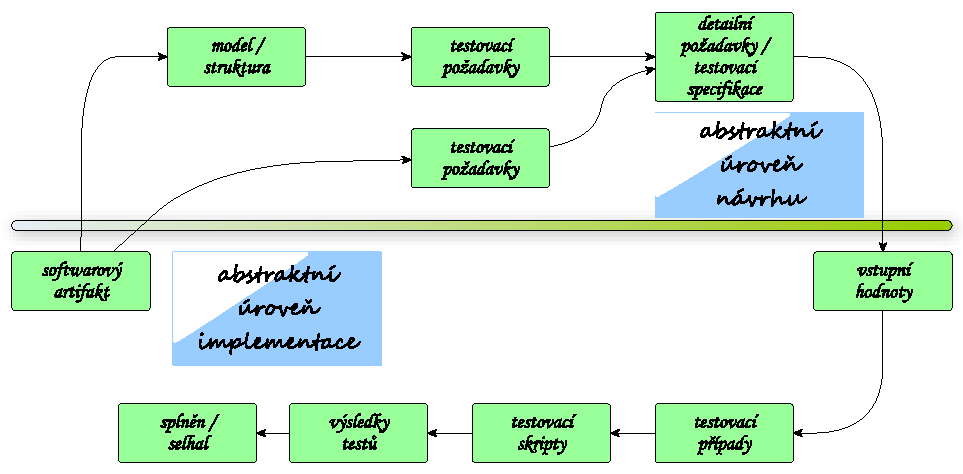
\includegraphics[width=130mm]{14/images/test-model}
\end{figure}

\paragraph{Návrh testování podle modelu}
\begin{itemize}[itemsep=0px]
\item definuj graf, definuj relace
\item navrhni testy pro pokrytí uzlů
\item navrhni testy pro pokrytí hran
\item otestuj všechny atributy
\item navrhni testy smyček
\end{itemize}

\paragraph{Kritéria pokrytí}
\begin{itemize}[itemsep=0px]
\item \textbf{Pokrytí řádek} - požaduje provedení každé řádky kódu alespoň jednou
\item \textbf{Pokrytí větví} - znamená, že podmínka každého větvení musí být alespoň jednou pravdivá a jednou nepravdivá
\item \textbf{Pokrytí podmínek} - zkontroluje všechny možné způsoby, za kterých daná podmínka je pravdivá či nepravdivá
\item \textbf{Úplné pokrytí cest} - vyžaduje provedení všech možných různých úplných cest (v praxi neproveditelné)
\end{itemize}

\subsection{Statická a dynamická analýza}
\textbf{Statická analýza} je model checking (viz následující otázka) a testování konečného automatu.

Analýza kódu, hledájí se v něm logické chyby jako např. nekonečný cyklus, nepoužívané proměnné, přiřazení místo porovnání atd. Řeší to např. pluginy do IDE (nebo IDE samotné).

\textbf{Dynamická analýza} je test běžící aplikace AUT=application under test. Třeba checkování použití paměti (Rational Purify, Boundchecker)

\subsection{Analýza toků řízení (metoda hlavních cest)}

\paragraph{Jednoduchá cesta} Cesta z $n_i$ do $n_j$ na které se žádný uzel neobjevuje více jak jedenkrát s vyjímkou, že počáteční a koncový uzel mohou být identické.

\paragraph{Hlavní cesta} Cesta z $n_i$ do $n_j$ je hlavní, jestliže je to jednoduchá cesta a není žádnou vlastní podcestou jakékoliv jiné jednoduché cesty (tj. je maximální).

\noindent Cílem je nalézt hlavní cesty. \textbf{Princip algoritmu:}

\begin{itemize}[itemsep=0px]
\item Nalezni cesty délky 0 (uzly).
\item Kombinuj cesty délky 0 do cest délky 1 (hrany).
\item Kombinuj cesty délky 1 do cest délky 2.
\item atd.
\end{itemize}

\subsection{Analýza datových toků (metoda du-cest)}
Tok datových hodnot: testy zajišťující, že hodnoty vzniklé na jednom místě jsou použity správně na jiných místech. 

\begin{itemize}[itemsep=0px]
\item \textbf{Definice} \textit{def}: místo, kde je hodnota proměnné uložena do paměti. 
\item \textbf{Užití} \textit{use}: místo, kde se přistupuje k hodnotě proměnné.
\item \textbf{DU páry def-use:} asociace určující přenosy hodnot. 
\end{itemize}

\paragraph{Formalizace}
\begin{itemize}[itemsep=0px]
\item V : množina proměnných asociovaná se softwarovým artefaktem. 
\item def : místo, kde je hodnota proměnné uložena do paměti
\item use : místo, kde se přistupuje k hodnotě proměnné
\item def (n) = podmnožina množiny proměnných $V$, které jsou definovány uzlem $n$
\item use (n) = podmnožina množiny proměnných $V$, které jsou použity v uzlu $n$
\item du(n, v) je množina všech du-cest vzhledem k proměnné $v$, která začíná v uzlu $n$
\end{itemize}

\subsection{Testování OO softwaru}

\paragraph{Anomálie DU párů}

Anomálie souvisí s děděním a polymorfismem.

Jsou třídy A $\leftarrow$ B.

\begin{itemize}[itemsep=0px]
\item \textbf{ITU} - inconsistent type use - nepřepisování ale volání parent metod, nejdřív použiju metody B, pak nějaké z A a pak opět B (A metody mohou něco nečekaně přepsat - přivézt objekt do stavu nekonzistentním s B).

\item \textbf{SDA} - state definition anomaly - přepisící metoda má jinou def množinu než přepisovaná (přepisující metody v B nenadefinují některé proměnné, které jsou definovány přepsanými metodami v A).

\item \textbf{SDIH} - podobné SDA ale potomek přepíše něco v prarodiči a rodič pak používá špatně definovanou proměnnou.

\item \textbf{ACB1} - přepis konstruktoru, potomek pak používá něco co není definováno.

\item \textbf{SVA} - přepsání metody v prarodiči, později rodič taky přepíše tu metodu a potomek začne volat rodiče, ne prarodiče
\end{itemize}

\paragraph{Testování párových sekvencí}

Typy testování: intra/inter metod a intra/inter tříd

Používá se k reprezentace interakce stavových prostorů, identifikace bodů integrace a testovacích požadavků. V softwarových artefaktech se hledají vazby last-def a firt-use po volání metody a uvnitř metody.

Testumeme, jak na sebe vzájemně působí metoda a instance vázaná na objekt o. Uvažují se metody které mohou být ve skutečnosti provedeny, testují se všechny vazby se všemi typy.
